\documentclass{article}
\usepackage{graphicx} % Required for inserting images
\usepackage{listings}
\usepackage{amsmath}
\usepackage{bm}
\usepackage{todonotes}
\usepackage{tikz}
\usepackage{hyperref}
\usepackage[english,capitalize,noabbrev]{cleveref}
\usepackage[\languagename,capitalize,noabbrev]{cleveref}
\usetikzlibrary{positioning, arrows.meta}


\begin{document}

%%%%%%%%%%%%%%%%%%%%%%%%%%%%%%%%%%%%%%%%%%%%%%%%%
%
%       Bitte hier die eigenen Daten eingeben
%       (für Generierung der Titelseite etc.)
%
%%%%%%%%%%%%%%%%%%%%%%%%%%%%%%%%%%%%%%%%%%%%%%%%%

\newcommand{\autor}{Nils Reck}% Vorname Name
\newcommand{\mnr}{2898155} % Matrikelnummer, bspw.: 12345

%%%%%%%%%%%%%%%%%%%%%%%%%%%%%%%%%% 
%
% Hier können weitere Autoren (und eine Gruppe) definiert werden. Diese können durch Anpassung der Titelseite.tex und der Erklaerung.tex berücksichtigt werden:
%
%\newcommand{\autorII}{Erika Musterfrau}% Vorname Name
%\newcommand{\mnrII}{54321} % Matrikelnummer, bspw.: 54321
%
%\newcommand{\gruppenr}{00}
%
%%%%%%%%%%%%%%%%%%%%%%%%%%%%%%%%%%

\newcommand{\betreuerI}{Dr. Carel van Niekerk} % Name betreuender Prof

\newcommand{\betreuerII}{Dr. Hsien-Chin Lin} % Name 2. Betreuer

\newcommand{\modulname}{Implementing Transformers} % Hier den Modulnamen eingeben

\newcommand{\projektname}{Project Report} % Hier den Belegtitel eingeben

\newcommand{\datum}{29.\,01.\,2025}

% Fakultät und Studiengang:

\newcommand{\fak}{Dialog Systems and Machine Learning} % Eingabe der Fakultät
\newcommand{\studiengang}{Computer Science, MSc} % Eingabe des Studiengangs


\begin{titlepage}
\begin{center}
\includegraphics[width=.9\textwidth]{figures/HHU_Logo_WortBildMarke} \par
\vspace{2.5cm}
\textsc{\LARGE Faculty \fak} \par
\vspace{1.5cm}
\textsc{\Large \modulname} \par
\vspace{3cm}
{ \huge \bfseries \projektname} \par
\vspace{1.5cm}
%%%%%%%%%%%%%%%%%%%%%%%%%%%%%%%%%%
\renewcommand{\arraystretch}{1.5}
%Entsprechend der Anzahl der Autoren anpassen bzw. Kommentarzeichen (%) entfernen
\begin{table}[h]
\large
    \centering
    \begin{tabular}{lll}
        &
        %\underline{Gruppe \gruppenr} % Gruppennummer
        & \\
        \emph{Author} % ggf. "Autoren"
        & \autor & \mnr \\
        %& \autorII & \mnrII \\
        %...
        \vspace{-0.5cm} \\
        \emph{Supervisors} & \betreuerI & \betreuerII 
    \end{tabular}
\end{table}
\renewcommand{\arraystretch}{1} \par
%%%%%%%%%%%%%%%%%%%%%%%%%%%%%%%%%%
\vfill
{\large \datum}
\end{center}
\end{titlepage}


\section{Introduction}

The Transformer model~\cite{vaswani2017attention} established the foundation for more performant and context-aware sequence transduction by removing the recurrent or convolutional means of previous state-of-the-art models.
This is mainly due to the Transformer's ability to process multiple sequences at once.
Up until today, the Transformer model remains the architecture of choice for top-performing large language models, like GPT-4o. \\
This report showcases my attempt to implement a custom Transformer model for a German-English translation task and aligns with the practicals conducted during the course.
In particular, it focuses on providing the reader with detailed knowledge about its components and their interplay, as well as my personal insights and struggles during development and training.
Thus, the report commences with a methodolgy section, explaining the modular components of a Transformer and the overall architecture.

% Study the model in the paper Attention is all you need. Write down the
% structurg of the proposed model.

\section{Methodology} 
However, before the model can process the input data, it has to be encoded in a numerical representation that the model can interpret.
For this, a shared tokenizer is trained over the source and target sequences, which maps a token (a word or subword) of a sequence to a number and vice versa. 

\todo[inline]{add info about alignment of sequences (maybe add to training section)}

\begin{figure}[h]
    \begin{center}
        \includegraphics[width=\textwidth]{figures/transformer.png}
    \end{center}
    \caption{The original transformer architecture, adapted from Vaswani et al.~\cite{vaswani2017attention}}\label{fig:transformer}
\end{figure}

\subsection{Embedding Layers} 
The embedding layer creates a \texttt{$d_{model}$}-dimensional vector representation for each encoded token of the input and target sequence. 
Cosistent with the original Transfromer architecture, we apply parameter sharing by using the same set of weights for both embedding layers and the pre-softmax linear transformation, which maps the embeddings back to their respective token index.
Sharing parameters between the encoder and decoder embedding layers offers several advantages.
First, it can significantly reduce the model size while maintaining model performance~\cite{press2017usingoutputembeddingimprove}.
Second, parmeter sharing reduces the degrees of freedom of the model, thus implicitly applying regularization by forcing different parts of the model to use the same parameters, preventing the model from overfitting.
Additionally, the efficiency of the model improves because shared parameters allow for faster updates and fewer memory operations.
Finally, by tying the input and output embeddings together, the model can enhance cross-lingual transfer learning, as aligned word representations across languages make it easier to generalize.\todo{delete last point?} \\
Unlike recurrent architectures, which process sequences step by step, the Transformer processes entire sequences in parallel. 
To compensate for the lack of sequence order awareness, the positional encoding layer enriches the representations with fixed positional information. \todo{How does the model differentiate between embedding and position?} \\
\todo[inline]{add formulars if space permits}

\subsection{Encoder Stack} 
The encoder consists of six identical layers, each designed to transform the input sequence into a context-rich representation.
Each layer comprises two sub-layers: a multi-head self-attention mechanism and a position-wise feed-forward network (see \cref{sec:ffn}), each followed by a residual connection~\cite{he2015deepresiduallearningimage} and layer normalization~\cite{ba2016layernormalization} (see \cref{sec:normalization}) to stabilize training and improve gradient flow.
Residual connections, defined as  \(y = \mathbf{x} + f(\mathbf{x})\), preserve the original signal while adding important features from multi-head attention or feed-forward layers, alleviating the problem of vanishing gradients during backpropagation.
If the transformation \(f(\mathbf{x})\) collapses to zero (e.g. due to all weights and biases being pushed to zero), the output reduces to \(y = \mathbf{x}\), ensuring that the original signal is preserved when the layer does not learn anything.
Residual connections can also be described by the residual mapping \(g(\mathbf{x}) = f(\mathbf{x}) - \mathbf{x}\), emphasizing that the network only needs to learn a small transformation when \(f(\mathbf{x})\) is close to the identity function.
Learning a function close to the identity function, residual blocks slightly refine existing features instead of learning full (high variance) functions from scratch. \\
Additionally, by focussing on small residuals \(g(\mathbf{x}) = f(\mathbf{x}) - \mathbf{x}\), the network increases the chance of generalizing better to unseen data, reducing overfitting.\todo{why?}

\subsection{Decoder Stack} 
The decoder also consists of six identical layers.
In addition to the two sub-layers of the encoder, it has a second multi-head attention mechanism over the outputs of the encoder.
Consistent with the encoder, residual connections and layer normalization are employed after each sub-layer.
In contrast to the multi-head self-attention layer in the encoder, the inputs to the attention mechanism in the decoder are masked such that the decoder cannot attend to future tokens.
This prevents the decoder from cheating by attending to tokens it has not yet seen.
Finally, the output of the decoder undergoes a linear transformation. After that, softmax is applied to convert the output into probabilities to predict the next token.

% Add how the heads are concatenated in attention
\subsection{Attention} 
The attention function injects contextual information about related tokens into each token's representation.
This process enables the model to capture dependencies between words, regardless of their position in the sequence. \\
The first step is to create the query(\(Q)\), key(\(K)\), and value(\(V)\) vectors from the encoder or decoder input vectors by multiplying them with three matrices that are learned during training.
These matrices must be learned in a way that they reflect meaningful similarity relationships in terms of attention. \\
According to \cref{eq:attention}, the attention function then first computes a score for each token in the sequence relative to every other token by taking the dot product of the query vector with the transposed key vector. 
\begin{equation}
    \text{Attention}(Q,K,V) = \text{softmax}\left(\frac{QK^T}{\sqrt{d_k}}\right)V
    \label{eq:attention}
\end{equation}
This computation, along with all other operations of the attention mechanism, is performed in parallel for all tokens in each sequence across the entire batch.
Next, the result is scaled by \(\sqrt{d_k}\) to avoid exploding gradients and improve stability.
Then a softmax function is applied to maintain relevant words, subside words we can mostly ignore, and prepare the output to be summed up.
Finally, by multiplying the softmax scores by \(V\) produces a new representation for each token.
While it retains most of its original structure, it is enriched with contextual information form the most relevant tokens for our translation task. \\
In the attention mechanism, we employ two types of masks; first, an attention mask to prevent the attention function from attending to padding tokens.
Second, a causal mask in the Masked Multi-Head Attention of the decoder to prevent our model from cheating by attending to future tokens during inference.

\subsection{Position-Wise Feed-Forward Networks} \label{sec:ffn}
\begin{equation}
	\text{FFN}(x) = \max(0, xW_1 + b_1)W_2 + b_2
\end{equation}
The FNN introduces a higher-dimensional space to explore combinations of features present in the token embeddings that it could not explore in the original embedding space.
That happens by the first linear transformation \(xW_1 + b_1\).
Next, ReLU, \(\max(0, xW_1 + b_1)\) introduces non-linearity (why does that help?) and helps prevent vanishing gradients (how?). 
The FFN has two linear layers of size \(\left(d_{\text{model}}, d_{\text{ffn}}\right)\) and \(\left(d_{\text{ffn}}, d_{\text{model}}\right)\), respecetively.
Finally, the non-linearly transformed representation is projected back into the original space, \(d_{\text{model}}\), such that it (what is it?) is forced to focus on the most significant feature combinations (bring examples).

\subsection{Normalization Layer} \label{sec:normalization}
Layer normalization is applied after each self-attention and feed-forward sublayer.
\begin{equation}
	\text{LayerNorm}(x) = \frac{x - \mu}{\sigma} \cdot \gamma + \beta
\end{equation}
Where \(x\) is the input vector, in our case the token embedding, \(\mu\) the mean of \(x\), calculated across the features, \(\sigma\) is the standard deviation, also calculated across the features:
\begin{align}
	\mu^l = \frac{1}{H} \sum_{i=1}^H a_i^l &   & \sigma^l = \sqrt{\frac{1}{H}\sum_{i=1}^H (a_i^l - \mu^l)^2} 
\end{align}
\(H\) is the number of features for each token representation, \(\gamma\) and \(\beta\) are optional, learnable parameters to scale and shift the normalized values. \\
In a transformer architecture, the layer normalization layer serves different purposes: it stabilizes training by normalizing the distributions of the layer inputs, thus preventing exploding or vanishing gradients, which would also have adverse, covariate effects on the surrounding layers in the forward and backward passes.
Additionally, contrary to batch normalization, layer normalization handles variations in sequence length better, since it computes the mean and variance along the features of the token and not across the individual features across the batch.

\begin{center}
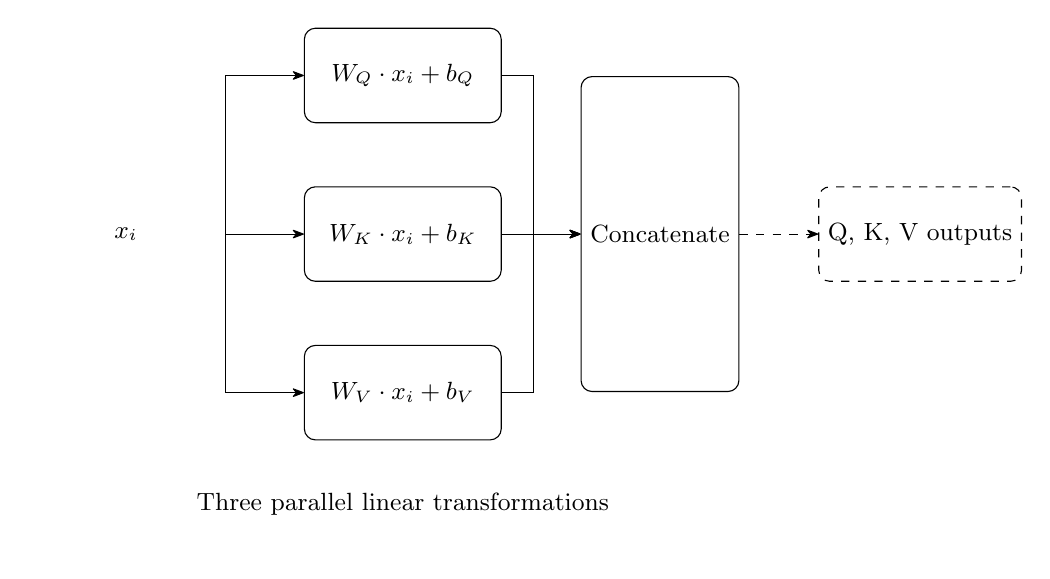
\begin{tikzpicture}[
		>={Stealth[round]}, % Arrow style
		node distance=2.5cm, % Distance between nodes
		every node/.style={draw, rounded corners, minimum width=2.5cm, minimum height=1.2cm, font=\small}
	]
			
	% Input node
	\node[draw=none] (input) {$x_i$};
			
	% Linear layer nodes
	\node[right=1cm of input] (K) {$W_K \cdot x_i + b_K$};
	\node[above=0.8cm of K] (Q) {$W_Q \cdot x_i + b_Q$};
	\node[below=0.8cm of K] (V) {$W_V \cdot x_i + b_V$};
			
	% Connect input to each linear layer
	\draw[->] (input.east) |- (Q.west);
	\draw[->] (input.east) |- (K.west);
	\draw[->] (input.east) |- (V.west);
			
	% Label nodes
	\node[below=0.2cm of V, draw=none] (labels) {Three parallel linear transformations};
			
	% Concatenate box with vertical text
	\node[draw, right=1cm of K, minimum width=1.2cm, minimum height=4cm, align=center] (concatBox) {Concatenate};
			
	% Connect linear layers to the concatenate box
	\draw[->] (Q.east) -- ++(0.4,0) |- (concatBox.west);
	\draw[->] (K.east) -- ++(0.4,0) |- (concatBox.west);
	\draw[->] (V.east) -- ++(0.4,0) |- (concatBox.west);
			
	% Dashed QKV outputs box centered vertically with Concatenate box
	\node[draw, dashed, right=1cm of concatBox, minimum width=2.5cm, minimum height=1.2cm, font=\small] (QKVBox) {Q, K, V outputs};
			
	% Arrow to QKV outputs
	\draw[->, dashed] (concatBox.east) -- (QKVBox.west);
			
\end{tikzpicture}
\end{center}

\section{Optimization Techniques}
\subsection{Learning Rate Scheduler}
\subsection{Optimizer}
% Study the AdamW optimiser used. Write down the update equations and explain
% the reasoning behind the bias correction and decoupled weight decay.

\section{Training}
% What went wrong during multiple iterations of training?
This section covers the training regime and a comparison between CPU and GPU training.
The code is available on GitLab\footnote{\url{https://git.hhu.de/nirec101/transformer_project}}.

\subsection{Data}
We train on the WMT 17 German-to-English dataset\footnote{\url{https://www.statmt.org/wmt17/translation-task.html}}, consisting of about 4.9 million sentence pairs after filtering out sequences exceeding 64 tokens in length.
To not inflict unnecessary load on the GPU during training, we preprocess the datasets beforehand.
The sequences are encoded using byte-pair encoding~\cite{britz2017massiveexplorationneuralmachine}, which has a shared source-target vocabulary of 50000 tokens.
We use only 5\% of the training data for benchmarking CPU vs. GPU performance with a batch size of 32 on both.
For the final model performance reported in \cref{sec:results}, however, we train on the entire dataset with a batch size of 256 sentence pairs.

\subsection{Training and Schedule}
We train our models on a single node with five processing cores and a single NVIDIA A100 GPU for around 170000 steps (10 epochs).
Since GPUs are optimized for parallel computation, they are well-suited for the highly parallel nature of sequence processing in Transformer models.
Unlike CPUs, which are designed for handling a wide range of sequential operations, the A100 distributes the workload across its many cores, consisting of 8192 FP32 CUDA cores and 432 Tensor cores\footnote{\url{https://images.nvidia.com/aem-dam/en-zz/Solutions/data-center/nvidia-ampere-architecture-whitepaper.pdf}}.
For benchmarking CPU vs. GPU performance under identical conditions, we use the exact same set of hyperparameters on both setups, with the CPU configuration consisting of five cores and 64GB of memory.
During full model training, each step took about 0.1 seconds, utilizing mixed precision.


\subsection{AdamW Optimizer}
In all the experiments, we use the AdamW optimizer~\cite{loshchilov2019decoupledweightdecayregularization} with \(\beta_1=0.9\), \(\beta_2=0.99\) and \(\epsilon=10^{-8}\).
This section elaborates the core differences between the Adam optimizer~\cite{kingma2017adammethodstochasticoptimization} used in the original Transformer architecture and AdamW.\\
Both, in Adam and AdamW, \cref{eq:mean_var} shows that the learning rate is adjusted for each parameter independently based on the history of gradients.
The running averages, \(m_{t-1}\) and \(v_{t-1}\), make it possible to include the history of the gradients in the calculation of the first and second moment:

% Equation 1: First moment estimate
\begin{equation}
\label{eq:mean_var}
m_t = \beta_1 m_{t-1} + (1 - \beta_1) g_t \text{,} \quad v_t = \beta_2 v_{t-1} + (1 - \beta_2) g_t^2
\end{equation}
The calculation of the first and second moment in this fashion ensures that parameters with larger gradient variances are updated more slowly than those with larger gradient variances to stabilize the optimization process. \\
The bias correction from \cref{eq:moments} is important because, without it, the first and second moments are biased toward zero at early time steps, because \(m_0\) and \(v_0\) are zero. Consequently, this results in overly careful parameter updates in the beginning, which hinder the performance and convergence of the training process. \\
% Equation 3: Bias-corrected moments
\begin{equation}
\hat{m}_t = \frac{m_t}{1 - \beta_1^t} \text{,} \quad \hat{v}_t = \frac{v_t}{1 - \beta_2^t}
\label{eq:moments}
\end{equation}
\\
In the original Adam, weight decay is added directly to the gradient. Consequently, this means that the weight decay term is included in the moment estimates (\(m_t\) and \(v_t\)). The AdamW optimizer circumvents this problem: The weight decay is applied directly to the weights after the gradient update, as shown in \cref{eq:weight_decay}:
% Equation 5: Weight decay
\begin{equation}
\label{eq:weight_decay}
\theta_t \leftarrow \theta_t - \eta \lambda \theta_t
\end{equation}
\\
\cref{eq:update} shows the complete parameter update for the AdamW optimizer, where the weight decay is decoupled from the gradient calculation.
% Equation 6: Parameter update
\begin{equation}
\label{eq:update}
\theta_{t+1} = \theta_t - \eta \left( \frac{\hat{m}_t}{\sqrt{\hat{v}_t} + \epsilon} \right) - \eta \lambda \theta_t
\end{equation}

\subsection{Estimation of Memory Requirements}
Estimating memory requirements involves accounting for not only the model parameters but also the optimizer states, activation storage during the forward and backward passes for proper gradient computation, and additional buffers used in matrix operations, softmax computations, etc.\\
PyTorch uses \texttt{float32} precision by default, meaning it uses 4 bytes to represent a single parameter.
The full Transformer model comprises \(\sim\) 95 million parameters, resulting in \(\sim\) 360MB of storage.
However, that does not account for the optimizer states, which contribute two extra values (first and second moment) per parameter (excluding bias terms), effectively tripling the memory requirements.
On top of that, the activations during the forward pass have to be considered, as well as the gradients for the backward pass, each contributing tensors of size \((256, 64, 512)\) for each layer.\\
For our model, this results in an approximate memory requirement of 6GB, which is consistent with the memory usage logs from training.
The tensor size is heavily sensible to the batch size, which could be empirically validated during training; a run with a larger batch size would crash with an out-of-memory error, even though theoretically, our GPUs have 40-80GB of VRAM, an issue to be further investigated.




\section{Results}\label{sec:results}

This section provides the results of the CPU vs. GPU comparison, as well as the performance of the Transformer model on the translation task.

\subsection{GPU versus CPU Training}

\cref{tab:comparison} illustrates the results of the performance comparison between CPU and GPU training.
The GPU significantly accelerates the overall training process by a factor of 8.07.
Accordingly, the GPU processes a single epoch, as well as a forward pass, faster by approximately the same margin.
The GPU achieves the most significant speed-up (20x) during the backward pass.
This highlights the GPU's superior efficiency in handling computationally expensive tasks, such as gradient computation, which heavily rely on parallelized matrix calculations.
Surprisingly, the GPU uses 38 times less memory per epoch compared to the CPU, which can mainly be attributed to the small batch size of 32 for both setups.\\
Due to approaching deadlines and long queues on the high performance cluster (HPC), I postpone further optimizations of the GPU codebase.
For instance, offloading BLEU score calculations to the CPU, combined with mixed-precision training and other optimizations, can approximately halve overall training time--a speedup that has been observed in practical 11.\\
\begin{table}[ht]
    \centering
    \begin{tabular}{lccc}
        \toprule
        \textbf{Metric} & \textbf{CPU} & \textbf{GPU} & \textbf{CPU to GPU Ratio} \\
        \midrule
        Training time (hours)       & 3.0017 & 0.3717 & 8.07 \\
        Avg. Epoch times (seconds)       & 2161.24 & 267.63 & 8.07 \\
        Avg. Forward pass times (seconds)& 0.0770 & 0.0088 & 8.75 \\
        Avg. Backward pass time (seconds)& 0.2020 & 0.0101 & 20 \\
        Avg. Single step time (seconds)  & 0.2790 & 0.0189 & 14.76  \\
        Allocated memory per epoch (MB)       & 32998.0  & 865.91 & 38.1 \\
        \bottomrule
    \end{tabular}
    \caption{Performance comparison of CPU vs. GPU}
    \label{tab:comparison}
\end{table}
While the performance benefits speak for themselves, GPU training entails some disadvantages.
Working on the HPC, I experienced long queues before the jobs could start, as well as complexity in setting up the code and accompanying libraries to run on the GPU nodes.
This results in longer feedback cycles because each attempt requires submitting a new job and waiting.
If errors occur, they only got discovered after the job queue processed the experiment, further extending debugging time.
Additionally, estimating the memory resources for optimizing throughput was time-consuming and often required trial and error, especially without easy access to a GPU for testing.

\clearpage
\subsection{Machine Translation}
\cref{fig:bleu} shows that on the WMT German-to-English translation task, the Transformer model reaches a BLEU score of around 0.34 with a length ratio of 0.99 on the validation set, which implies solid, coherent translations.
Training took approximately 11.5 hours.


\begin{figure}[ht]
    \begin{center}
        \includegraphics[width=\textwidth]{figures/bleu_score_val_20250129_142747.png}
    \end{center}
    \caption{The BLEU score is calculated on the validation set after each epoch. It approaches a value of around 0.34.}
    \label{fig:bleu}
\end{figure}
Word count: 2282


\begin{enumerate}
	\item Make sure you understand the embeddings of the input. Explain why we need the position of input characters in the embedding.
	\item Make sure you understand the role of the two different masks in the attention mechanism. Explain the role of each mask in your own words.
	\item The model starts with a Query (Q) for the current position. For example, if the model predicts the next token for the word "cat", the Query is derived from the representation of "cat".
\end{enumerate}

\section{Questions}
\subsection{Practical 4}
\begin{enumerate}
	\item Wich dimension do the word embeddings need to have?
	\item Why do values have a different dimension \(d_v\), compared to queries and keys \(d_k \), wrt the linear projection in mha?
    \item How does the model differentiate between embedding and positional encoding?
\end{enumerate}
\subsection{Practical 5}
\begin{enumerate}
	\item Why is it called encoder/decoder?
\end{enumerate}
\begin{enumerate}
	\item Do we put the tokenizer in the \lstinline{TranslationDataset} class?
	\item What is the word embedding dimension?
\end{enumerate}


\clearpage


\todo[inline]{Where do we apply dropout?}
\todo[inline]{What are learnable parameters in a transformer model?}
\todo[inline]{Inclued questions from tests}

\clearpage



\clearpage
\bibliography{references}
%% Depending on Language, use German alphadin or original alpha
\iflanguage{ngerman}{
  \bibliographystyle{alphadin}
}{
  \bibliographystyle{alpha}
}

\end{document}
